\documentclass[12pt,a4paper]{article}
\usepackage[margin=2cm]{geometry}
\usepackage{graphicx}
\usepackage{xcolor}
\usepackage{listings}
\usepackage{booktabs}
\usepackage{hyperref}
\usepackage{float}
\usepackage{enumitem}
\usepackage{fancyhdr}
\usepackage{titlesec}
\usepackage{caption}
\usepackage{array}
\usepackage[utf8]{inputenc}
\usepackage[T1]{fontenc}
\usepackage{amssymb}
\setlength{\headheight}{14pt}
\addtolength{\topmargin}{-2pt}

\definecolor{codeblue}{HTML}{1E40AF}
\definecolor{codebg}{HTML}{F1F5F9}
\definecolor{accent}{HTML}{6366F1}
\definecolor{darkbg}{HTML}{0F172A}

\lstset{
  backgroundcolor=\color{codebg},
  basicstyle=\ttfamily\small,
  breaklines=true,
  frame=single,
  rulecolor=\color{gray!30},
  keywordstyle=\color{codeblue}\bfseries,
  stringstyle=\color{teal},
  commentstyle=\color{gray},
  language=Python,
  showstringspaces=false,
  numbers=left,
  numberstyle=\tiny\color{gray},
  tabsize=2,
  literate={á}{{\'a}}1 {é}{{\'e}}1 {í}{{\'i}}1 {ó}{{\'o}}1 {ú}{{\'u}}1
}

\pagestyle{fancy}
\fancyhf{}
\fancyhead[L]{\small 40\_CS4032 NLP -- Individual Assignment 02}
\fancyhead[R]{\small Vinusha Rathnayaka}
\fancyfoot[C]{\thepage}

\titleformat{\section}{\Large\bfseries\color{accent}}{}{0em}{}[\color{accent}\titlerule]
\titleformat{\subsection}{\large\bfseries\color{darkbg}}{}{0em}{}

\begin{document}

% ===== TITLE PAGE =====
\begin{titlepage}
\centering
\vspace*{2cm}
{\Huge\bfseries\color{accent} Offline Intelligent Sinhala\\Open-Ended Answer Scorer\par}
\vspace{0.5cm}
{\Large History of Sri Lanka -- Anuradhapura Period\par}
\vspace{1.5cm}
{\large\bfseries Module: 40\_CS4032 Natural Language Processing\par}
{\large Individual Assignment 02\par}
\vspace{1cm}
\rule{0.6\textwidth}{0.5pt}\par
\vspace{1cm}
{\large\bfseries Student:} Vinusha Rathnayaka\par
\vspace{0.5cm}
{\large\bfseries Technology Stack:}\par
OLLAMA + RAG + Ontology + Agent Architecture\par
\vspace{0.5cm}
{\large\bfseries Scope:} Option 1 -- Ancient Sri Lanka (Anuradhapura Period)\par
\vspace{2cm}
\begin{tabular}{ll}
\toprule
Component & Technology \\
\midrule
LLM & OLLAMA (SinLlama / llama3) \\
RAG & ChromaDB + MiniLM-L12-v2 \\
Ontology & Owlready2 (OWL) \\
UI & Streamlit \\
Mode & Fully Offline \\
\bottomrule
\end{tabular}
\vfill
{\large \today\par}
\end{titlepage}

\tableofcontents
\newpage

% ===== SECTION 1 =====
\section{Problem Setup \& History Scope}

This system is a fully \textbf{offline} intelligent scorer for Sinhala open-ended answers about the \textbf{Anuradhapura Period} of Sri Lankan history.

\subsection{Selected Scope: Ancient Sri Lanka (Anuradhapura Period)}
\begin{itemize}[leftmargin=*]
  \item \textbf{Administration} -- Royal governance, provincial and village-level systems
  \item \textbf{Irrigation/Civilization} -- Tanks (wewa), canals, agricultural engineering
  \item \textbf{Buddhism \& Culture} -- Introduction of Buddhism, stupas, monastic orders
  \item \textbf{Notable Rulers/Events} -- Dutugemunu, Dhatusena, Vasabha, Mahasena
  \item \textbf{Decline} -- South Indian invasions, fall of Anuradhapura, shift to Polonnaruwa
\end{itemize}

The system grades each answer out of \textbf{20 marks} using structured marking guides and produces \textbf{explainable score breakdowns} with Sinhala justifications.

% ===== SECTION 2 =====
\section{System Architecture -- Operational Flow Chart}

% ADD YOUR FLOWCHART IMAGE HERE:
\begin{figure}[H]
  \centering
  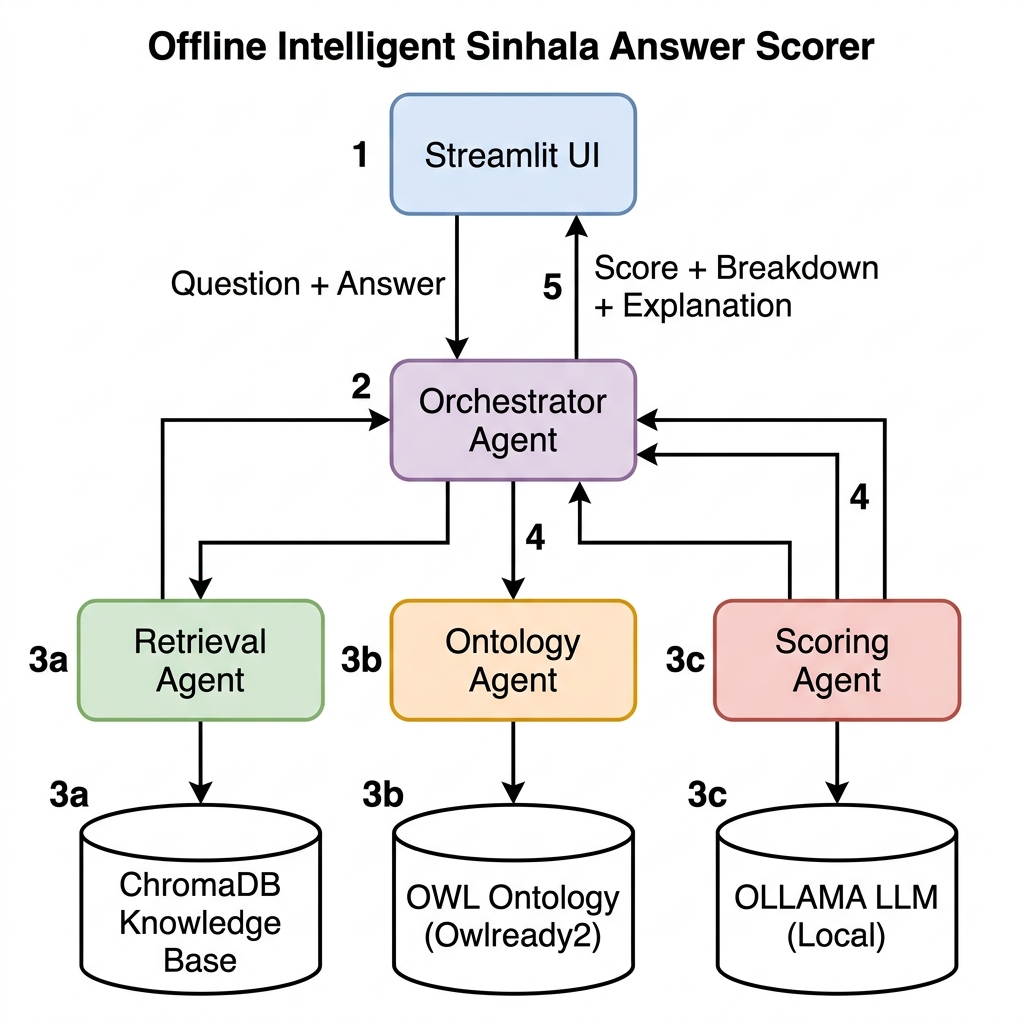
\includegraphics[width=0.85\textwidth]{report_screenshots/flowchart.png}
  \caption{System Architecture Flowchart}
\end{figure}

% ADD YOUR AGENT WORKFLOW IMAGE HERE:
\begin{figure}[H]
  \centering
  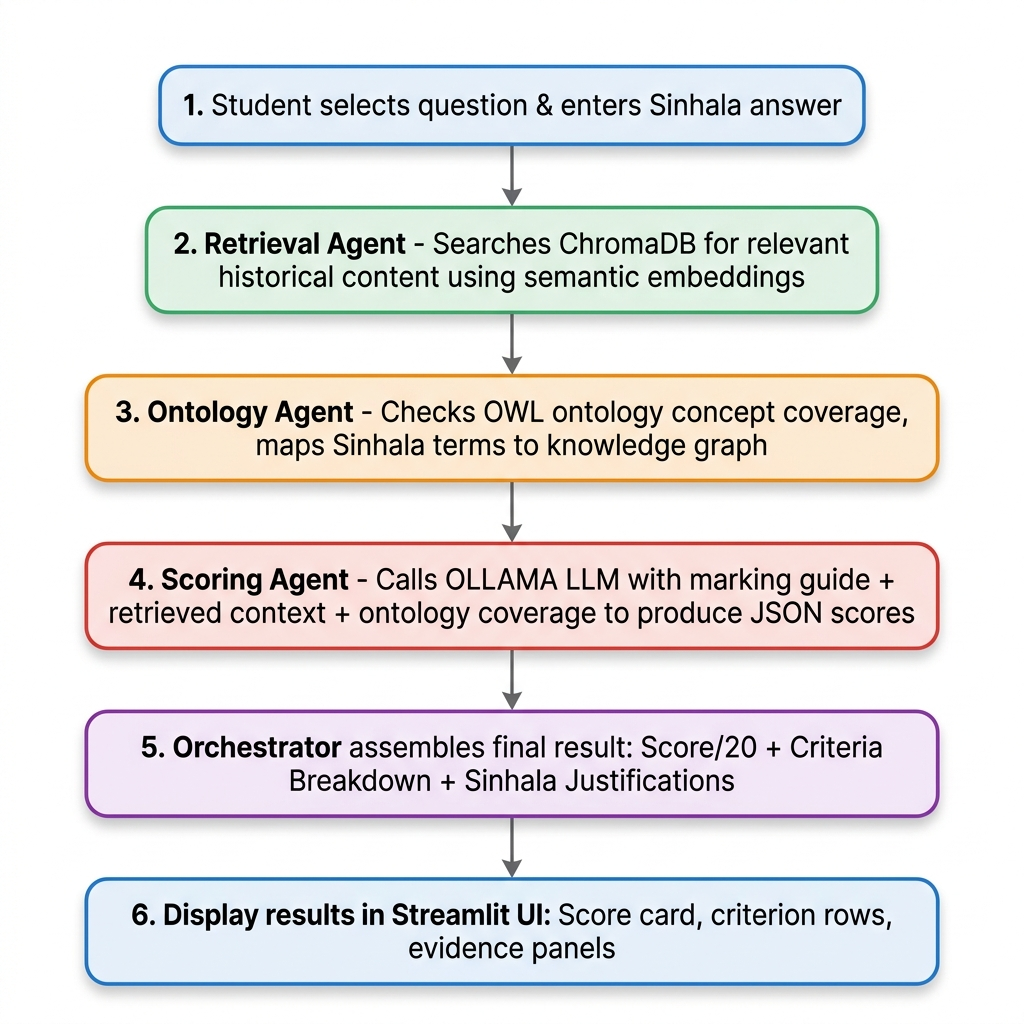
\includegraphics[width=0.7\textwidth]{report_screenshots/agent_workflow.png}
  \caption{Agent-Based Scoring Pipeline}
\end{figure}

\subsection{Workflow Steps}
\begin{table}[H]
\centering
\begin{tabular}{clp{9cm}}
\toprule
\textbf{Step} & \textbf{Agent} & \textbf{Action} \\
\midrule
1 & UI $\rightarrow$ Orchestrator & User selects question, enters Sinhala answer \\
2 & Retrieval Agent & Semantic search over ChromaDB knowledge base \\
3 & Ontology Agent & Concept coverage check against OWL ontology \\
4 & Scoring Agent & LLM evaluation via OLLAMA with all context \\
5 & Orchestrator $\rightarrow$ UI & Assembles score + breakdown + explanations \\
\bottomrule
\end{tabular}
\caption{Step-by-step operational workflow}
\end{table}

\subsection{Architecture Code -- Orchestrator}
\begin{lstlisting}[caption={Orchestrator workflow (orchestrator.py)}]
class OrchestratorAgent:
    def grade_answer(self, question_id, question_text,
                     student_answer, progress_callback=None):
        # STEP 1: Retrieval Agent
        retrieval_result = self.retrieval_agent.retrieve(
            question_text, student_answer)
        retrieved_context = self.retrieval_agent \
            .get_context_for_scoring(question_text, student_answer)

        # STEP 2: Ontology Agent
        ontology_result = self.ontology_agent.analyze(
            question_id, student_answer)
        ontology_coverage = self.ontology_agent \
            .get_coverage_summary(question_id, student_answer)

        # STEP 3: Scoring Agent (LLM with all context)
        scoring_result = self.scoring_agent.score(
            question_id=question_id,
            student_answer=student_answer,
            retrieved_context=retrieved_context,
            ontology_coverage=ontology_coverage,
            ontology_context=ontology_context)

        # STEP 4: Assemble final result
        return final_result
\end{lstlisting}

% ===== SECTION 3 =====
\section{Question Set \& Marking Guides (5 Questions)}

All 5 questions are in Sinhala, each graded out of 20 marks.

\subsection{Q1: Irrigation Civilization (Jalasha Shishtacharaya)}
\textbf{Question:} Discuss the water supply system of the Anuradhapura Kingdom in detail. Explain the key tanks, canal systems, and their impact on agriculture. \textit{(Asked in Sinhala)}

\begin{table}[H]
\centering
\begin{tabular}{clc}
\toprule
\# & Criterion & Marks \\
\midrule
1 & Key Tanks Identification (Abhaya, Tissa, Nuwara, Kala, Minneriya) & 5 \\
2 & Canal Systems Description (Jaya Ganga / Yoda Ela) & 4 \\
3 & Linking Irrigation to Agriculture & 4 \\
4 & Tank Builders (Vasabha, Mahasena, Dhatusena) & 4 \\
5 & Overall Quality \& Coherence & 3 \\
\midrule
  & \textbf{Total} & \textbf{20} \\
\bottomrule
\end{tabular}
\end{table}

\subsection{Q2: Introduction of Buddhism (Budu Dahama)}
\textbf{Question:} Explain how Buddhism was introduced to Sri Lanka and its impact on Anuradhapura society and culture. \textit{(Asked in Sinhala)}

\begin{table}[H]
\centering
\begin{tabular}{clc}
\toprule
\# & Criterion & Marks \\
\midrule
1 & Mahinda Thero's Mission, Ashoka, Devanampiya Tissa & 5 \\
2 & Key Buddhist Sites (Thuparamaya, Sri Maha Bodhi, Ruwanwelisaya) & 4 \\
3 & Three Monastic Fraternities (Mahavihara, Abhayagiri, Jetavana) & 4 \\
4 & Social \& Cultural Impact & 4 \\
5 & Overall Quality \& Coherence & 3 \\
\midrule
  & \textbf{Total} & \textbf{20} \\
\bottomrule
\end{tabular}
\end{table}

\subsection{Q3: Key Rulers \& Contributions (Pradhana Rajawarun)}
\textbf{Question:} Select three key rulers of the Anuradhapura era and discuss their contributions. \textit{(Asked in Sinhala)}

\begin{table}[H]
\centering
\begin{tabular}{clc}
\toprule
\# & Criterion & Marks \\
\midrule
1 & Correctly Identifying 3 Rulers with Reign Periods & 5 \\
2 & Military Achievements (e.g., Dutugemunu vs Elara) & 4 \\
3 & Infrastructure Contributions & 4 \\
4 & Religious \& Cultural Patronage & 4 \\
5 & Overall Quality \& Coherence & 3 \\
\midrule
  & \textbf{Total} & \textbf{20} \\
\bottomrule
\end{tabular}
\end{table}

\subsection{Q4: Administrative System (Paripalana Kramaya)}
\textbf{Question:} Describe the administrative structure of the Anuradhapura Kingdom. \textit{(Asked in Sinhala)}

\begin{table}[H]
\centering
\begin{tabular}{clc}
\toprule
\# & Criterion & Marks \\
\midrule
1 & King's Supreme Authority \& Citadel & 4 \\
2 & Provincial Administration (Uvarajas, Ratas) & 4 \\
3 & Village-Level Administration (Gamikas) & 4 \\
4 & Law, Taxation, Water Distribution Management & 4 \\
5 & Overall Quality \& Coherence & 4 \\
\midrule
  & \textbf{Total} & \textbf{20} \\
\bottomrule
\end{tabular}
\end{table}

\subsection{Q5: Decline of Anuradhapura (Parihaniya)}
\textbf{Question:} Discuss the factors that led to the decline of the Anuradhapura Kingdom. \textit{(Asked in Sinhala)}

\begin{table}[H]
\centering
\begin{tabular}{clc}
\toprule
\# & Criterion & Marks \\
\midrule
1 & South Indian Invasions (Chola, Pandya) & 5 \\
2 & Internal Conflicts \& Succession Disputes & 4 \\
3 & Mahinda V's Capture \& Fall (1017 CE) & 4 \\
4 & Shift to Polonnaruwa \& Strategic Reasons & 4 \\
5 & Overall Quality \& Coherence & 3 \\
\midrule
  & \textbf{Total} & \textbf{20} \\
\bottomrule
\end{tabular}
\end{table}

% ===== SECTION 4 =====
\section{RAG Implementation}

\subsection{Knowledge Base Documents}
\begin{table}[H]
\centering
\begin{tabular}{llr}
\toprule
\textbf{File} & \textbf{Topic} & \textbf{Size} \\
\midrule
irrigation.txt & Tanks, canals, agriculture & 4,467 B \\
buddhism.txt & Buddhism introduction \& impact & 5,167 B \\
rulers.txt & Key rulers \& contributions & 5,081 B \\
administration.txt & Administrative systems & 2,549 B \\
decline.txt & Fall of Anuradhapura & 3,453 B \\
\bottomrule
\end{tabular}
\caption{Sinhala knowledge base documents (all written in Sinhala)}
\end{table}

\subsection{Retrieval Pipeline}
\begin{lstlisting}[caption={Knowledge base setup (setup\_kb.py)}]
# Offline multilingual embedding model
model = SentenceTransformer(
    "paraphrase-multilingual-MiniLM-L12-v2")

# Paragraph-aware chunking
def chunk_text(text, chunk_size=500, overlap=100):
    paragraphs = [p.strip()
        for p in text.split('\n\n') if p.strip()]
    return chunks

# ChromaDB persistent storage with cosine similarity
client = chromadb.PersistentClient(path=CHROMA_DB_DIR)
collection = client.create_collection(
    name="sinhala_history",
    metadata={"hnsw:space": "cosine"})
collection.add(embeddings=embeddings,
    documents=chunks, ids=ids, metadatas=metadatas)
\end{lstlisting}

\subsection{Retrieval Agent}
\begin{lstlisting}[caption={Retrieval Agent (retrieval\_agent.py)}]
class RetrievalAgent:
    def retrieve(self, question, student_answer,
                 top_k=5):
        query_text = f"{question} {student_answer[:200]}"
        query_embedding = self.embedding_model \
            .encode(query_text).tolist()
        results = self.collection.query(
            query_embeddings=[query_embedding],
            n_results=top_k,
            include=["documents","metadatas","distances"])
        return formatted_results
\end{lstlisting}

Retrieved context is \textbf{directly injected} into the scoring prompt, ensuring the LLM grades based on verified factual content.

% ===== SECTION 5 =====
\section{Ontology Implementation}

% ADD YOUR ONTOLOGY DIAGRAM HERE:
\begin{figure}[H]
  \centering
  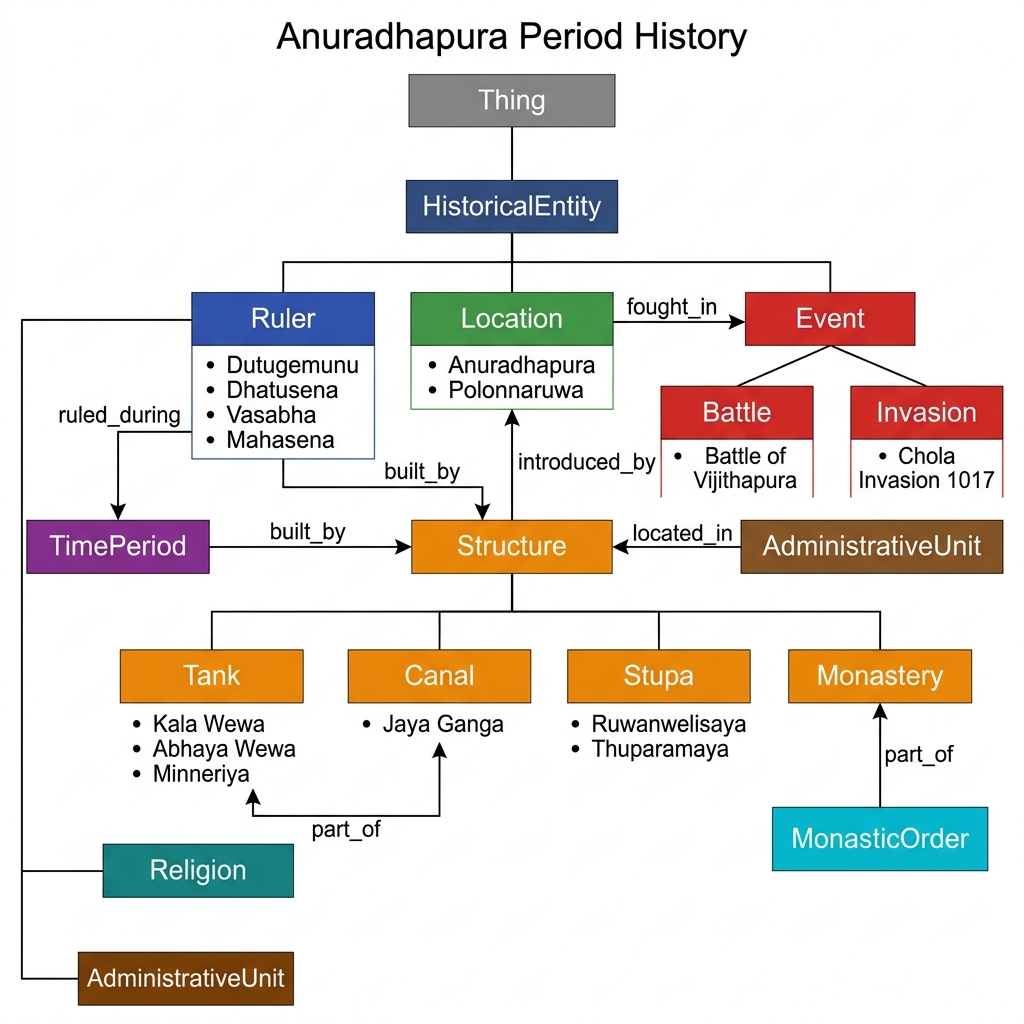
\includegraphics[width=0.8\textwidth]{report_screenshots/ontology_diagram.png}
  \caption{OWL Ontology Class Hierarchy}
\end{figure}

\subsection{OWL Ontology Structure}
Built using \textbf{Owlready2}, the ontology contains:
\begin{itemize}[leftmargin=*]
  \item \textbf{12+ Classes:} HistoricalEntity, Ruler, Location, Structure, Tank, Canal, Stupa, Monastery, Event, Battle, Invasion, MonasticOrder, TimePeriod, Religion, AdministrativeUnit
  \item \textbf{9 Object Properties:} built\_by, ruled\_during, located\_in, part\_of, introduced\_by, associated\_with, fought\_in, succeeded\_by, founded\_by
  \item \textbf{4 Data Properties:} reign\_start, reign\_end, significance\_si, significance\_en
  \item \textbf{30+ Individuals} with Sinhala significance annotations
\end{itemize}

\begin{lstlisting}[caption={Ontology creation (create\_ontology.py)}]
# Classes hierarchy
class HistoricalEntity(Thing): pass
class Ruler(HistoricalEntity): pass
class Structure(HistoricalEntity): pass
class Tank(Structure): pass
class Canal(Structure): pass

# Object Properties with domain/range
class built_by(ObjectProperty):
    domain = [Structure]; range = [Ruler]
class ruled_during(ObjectProperty):
    domain = [Ruler]; range = [TimePeriod]

# Individuals with Sinhala significance
dhatusena = Ruler("Dhatusena")
dhatusena.reign_start = "455 CE"
dhatusena.significance_si = "[Sinhala significance]"

kala_wewa = Tank("Kala_Wewa")
kala_wewa.built_by = [dhatusena]
\end{lstlisting}

\subsection{Concept Coverage Verification}
\begin{lstlisting}[caption={Ontology concept verification (ontology\_loader.py)}]
def verify_concept_coverage(self, answer_text,
                            question_id):
    # Sinhala term mapping for fuzzy matching
    name_map = {
        "Kala_Wewa": ["kala wewa", "kalawewa"],
        "Dhatusena": ["dhatusena"],
        "Jaya_Ganga": ["jaya ganga", "yoda ela"],
    }
    for concept_name in expected_concepts:
        is_found = any(
            term.lower() in answer_text.lower()
            for term in search_terms)
    return {
        "coverage_percentage": coverage_pct,
        "found_concepts": found,
        "missing_concepts": missing
    }
\end{lstlisting}

% ===== SECTION 6 =====
\section{Agent-Based Architecture}

\begin{table}[H]
\centering
\begin{tabular}{lll}
\toprule
\textbf{Agent} & \textbf{File} & \textbf{Responsibility} \\
\midrule
OrchestratorAgent & orchestrator.py & Coordinates full workflow \\
RetrievalAgent & retrieval\_agent.py & ChromaDB semantic search \\
OntologyAgent & ontology\_agent.py & Concept coverage verification \\
ScoringAgent & scoring\_agent.py & LLM-based evaluation via OLLAMA \\
\bottomrule
\end{tabular}
\caption{Agent responsibilities}
\end{table}

\subsection{Reliability Features}
\begin{itemize}[leftmargin=*]
  \item \textbf{Error Isolation:} Each agent wrapped in try/except; partial failures don't crash the system
  \item \textbf{Progress Tracking:} Real-time workflow logging with timestamps displayed in UI
  \item \textbf{Score Validation:} Awarded marks capped to max\_marks per criterion, ensured non-negative
  \item \textbf{Fallback Mechanism:} If LLM JSON parsing fails, fallback response is generated
\end{itemize}

% ===== SECTION 7 =====
\section{Explainable Scoring}

\subsection{LLM Prompt Engineering}
\begin{lstlisting}[caption={Scoring system prompt (scoring\_agent.py)}]
def _build_system_prompt(self):
    return """You are an expert Sinhala History teacher.
    RULES:
    1. Evaluate EACH criterion separately
    2. Assign score 0 to max_marks per criterion
    3. Provide Sinhala justification for each score
    4. Use retrieved context and ontology to verify
    5. Response MUST be valid JSON"""
\end{lstlisting}

\subsection{JSON Score Output Format}
\begin{lstlisting}[language={}]
{
  "criteria_scores": [
    {
      "criterion_name": "Key Tanks Identification",
      "max_marks": 5,
      "awarded_marks": 4,
      "justification_si": "[Sinhala justification
        explaining why marks were awarded/deducted]"
    }
  ],
  "total_score": 16,
  "total_max": 20,
  "overall_feedback_si": "[Overall Sinhala feedback]"
}
\end{lstlisting}

\subsection{Response Parsing \& Validation}
\begin{lstlisting}[caption={Score parsing with validation}]
def _parse_response(self, response, guide):
    json_match = re.search(r'\{[\s\S]*\}', response)
    parsed = json.loads(json_match.group())
    for i, score_item in enumerate(criteria_scores):
        max_marks = guide["criteria"][i]["max_marks"]
        awarded = min(score_item.get(
            "awarded_marks", 0), max_marks)
        awarded = max(awarded, 0)  # Non-negative
\end{lstlisting}

% ===== SECTION 8 =====
\section{Streamlit UI \& Usability}

% ADD YOUR UI SCREENSHOT HERE:
\begin{figure}[H]
  \centering
  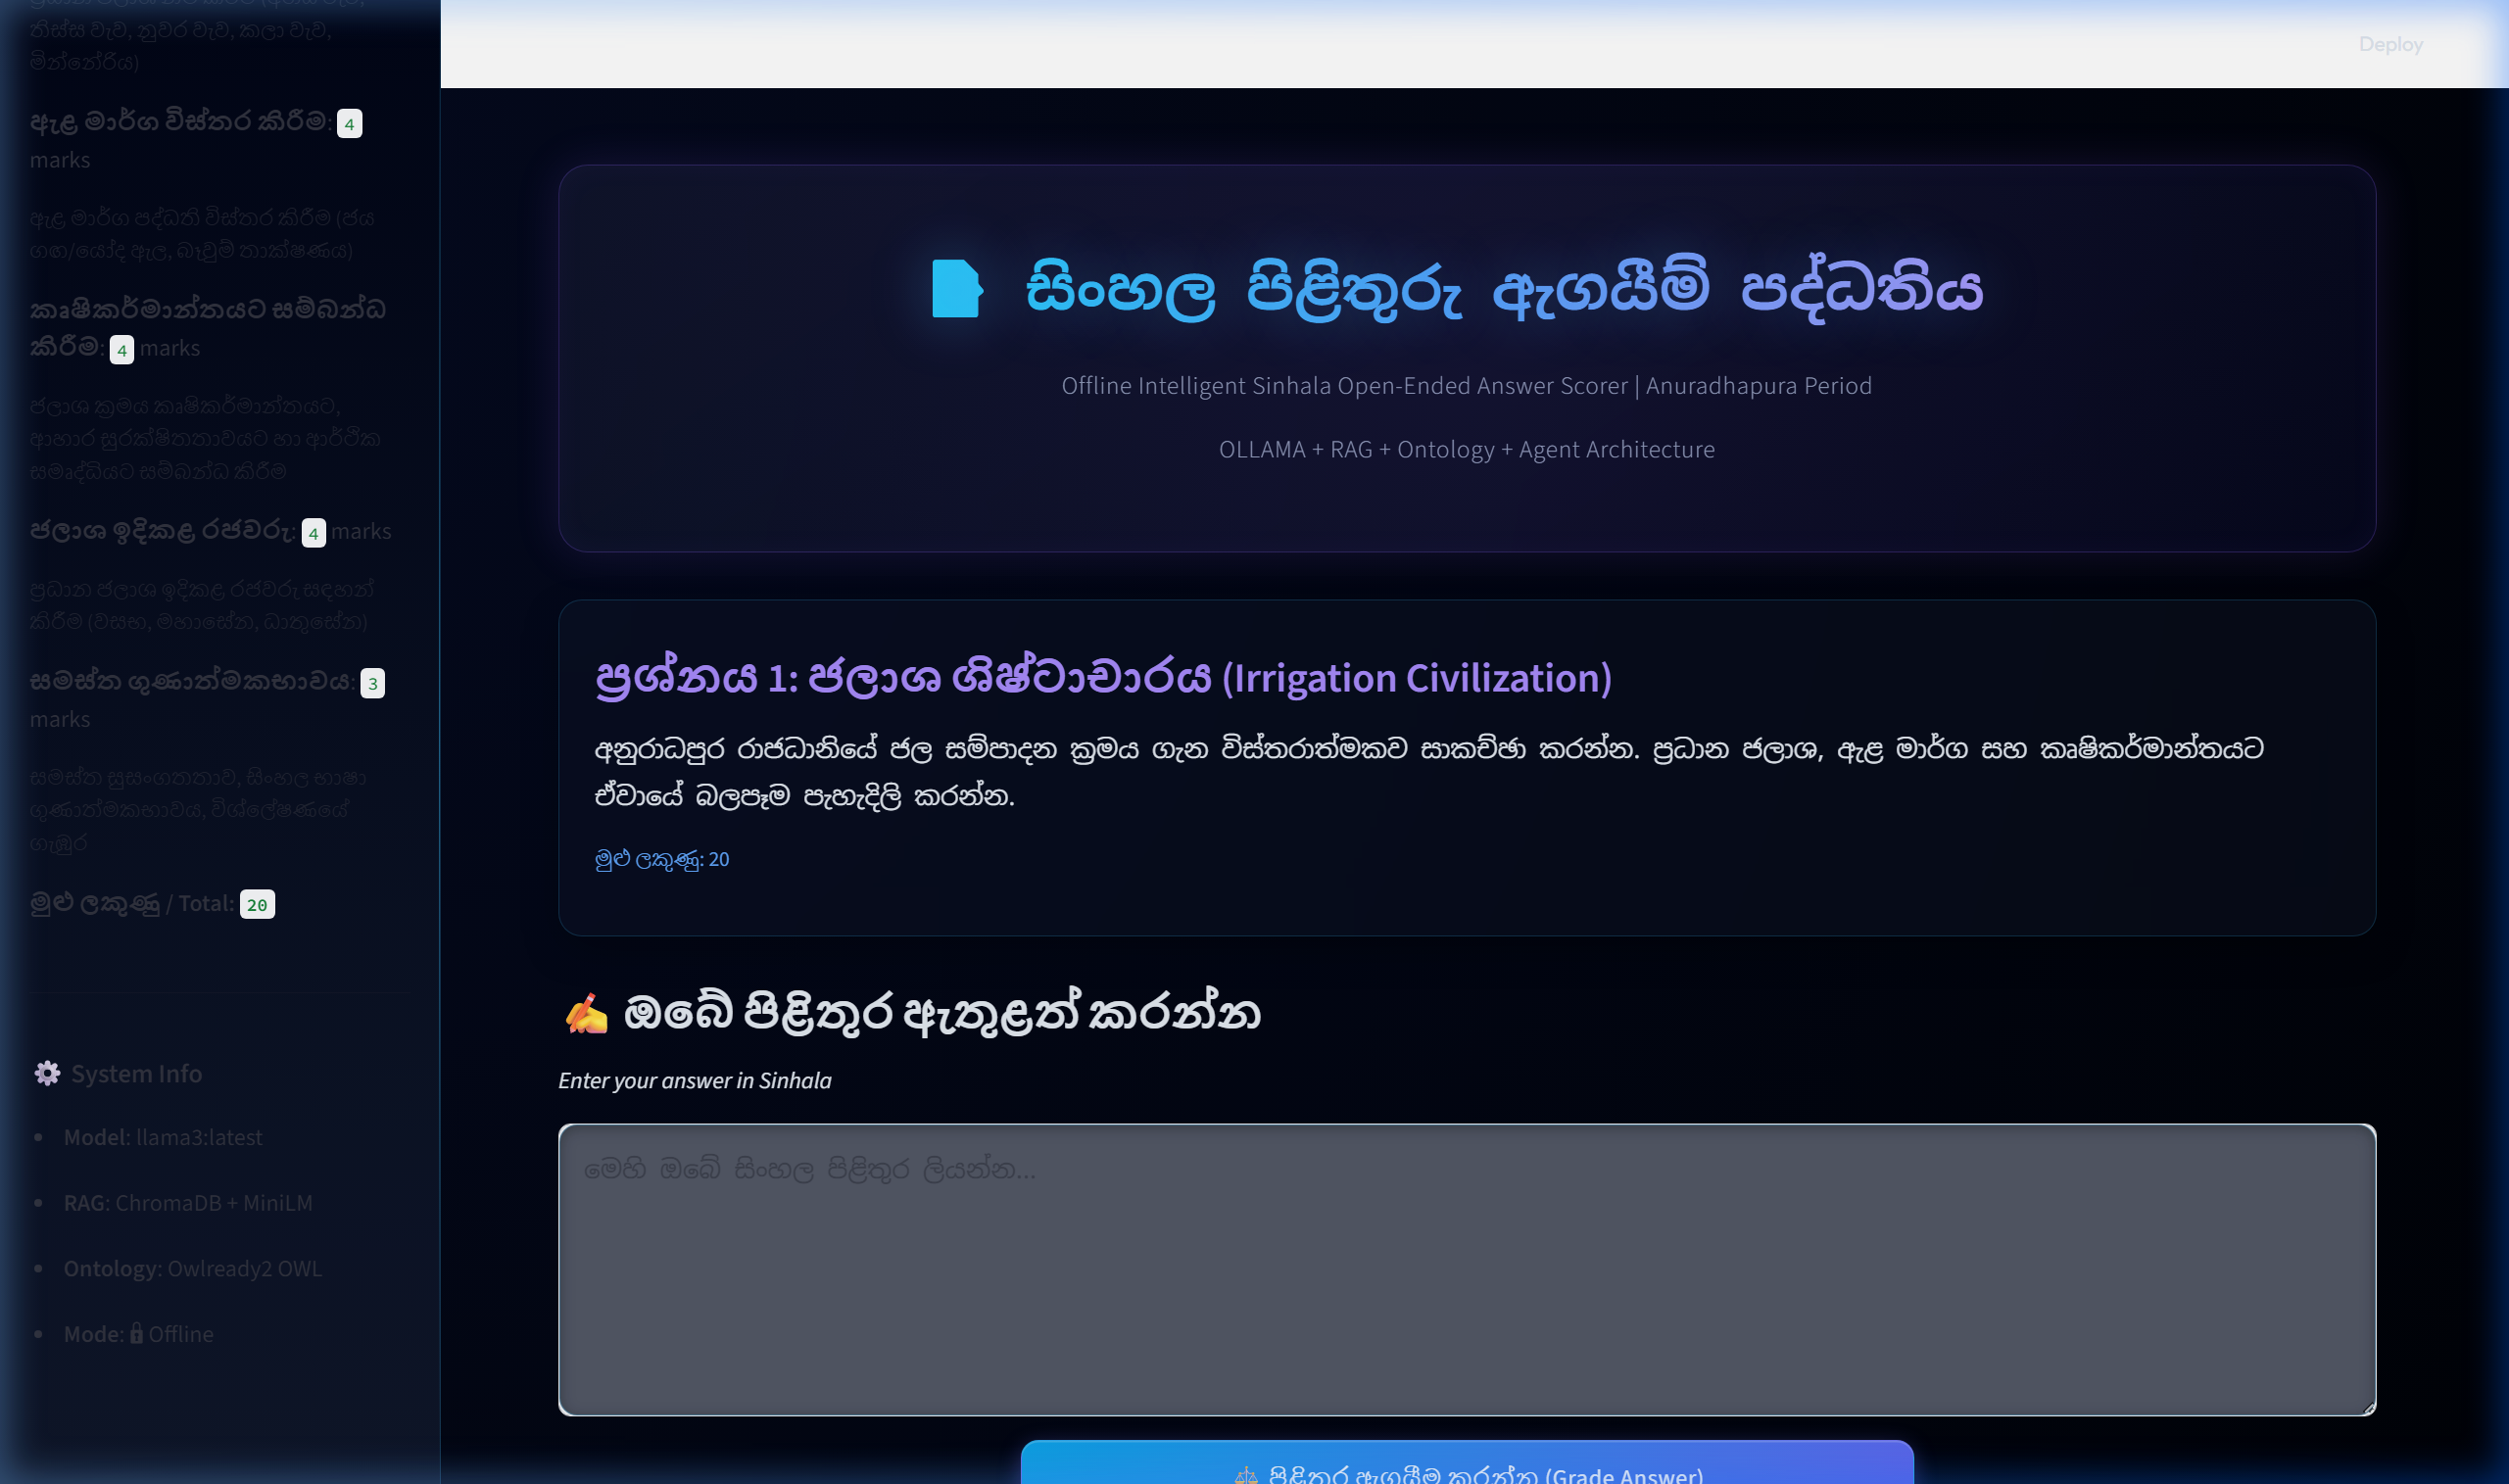
\includegraphics[width=0.9\textwidth]{report_screenshots/ui_main.png}
  \caption{Streamlit UI -- Main Interface}
\end{figure}

\subsection{Interface Components}
\begin{itemize}[leftmargin=*]
  \item \textbf{Sidebar:} Question selector dropdown, marking guide display, system info panel
  \item \textbf{Main Area:} Question display (glass-card design), Sinhala text input, grade button
  \item \textbf{Results:} Score card with performance badge, color-coded criterion rows with Sinhala justifications, overall feedback, expandable evidence panels
\end{itemize}

\begin{lstlisting}[caption={UI code excerpt (app.py)}]
# Sidebar - Question selection
with st.sidebar:
    questions = get_all_questions()
    selected = st.selectbox(
        "Select Question:", options=list(questions))
    for c in guide["criteria"]:
        st.markdown(f"**{c['name']}**: "
                    f"`{c['max_marks']}` marks")

# Answer input
student_answer = st.text_area(
    label="Student Answer", height=200,
    placeholder="Enter Sinhala answer here...")

# Grade button triggers orchestrator
if grade_button:
    orchestrator = get_orchestrator()
    result = orchestrator.grade_answer(
        question_id=selected_qid,
        question_text=guide["question"],
        student_answer=student_answer)
\end{lstlisting}

% ===== SECTION 9 =====
\section{Offline Operation}

\begin{table}[H]
\centering
\begin{tabular}{ll}
\toprule
\textbf{Component} & \textbf{Offline Mechanism} \\
\midrule
LLM Inference & OLLAMA on localhost:11434 \\
Embeddings & MiniLM-L12-v2 cached locally \\
Vector Store & ChromaDB persistent on disk \\
Ontology & Local OWL file (anuradhapura.owl) \\
Knowledge Base & 5 local Sinhala text files \\
UI & Streamlit on localhost:8501 \\
\bottomrule
\end{tabular}
\caption{Offline operation -- all components local}
\end{table}

\begin{lstlisting}[caption={Configuration (config.py)}]
OLLAMA_MODEL = "hf.co/SanudaDev/SinLlama-GGUF"
OLLAMA_BASE_URL = "http://localhost:11434"
EMBEDDING_MODEL = "paraphrase-multilingual-MiniLM-L12-v2"
LLM_TEMPERATURE = 0.1  # Low for consistent scoring
LLM_NUM_CTX = 4096
\end{lstlisting}

% ===== SECTION 10 =====
\section{Project Structure}

\begin{lstlisting}[language={},frame=single]
NLP II/
  app.py                 # Streamlit UI (638 lines)
  config.py              # Centralized configuration
  requirements.txt       # Dependencies
  setup_kb.py            # Knowledge base builder
  test_pipeline.py       # End-to-end test script
  agents/
    orchestrator.py      # Workflow coordinator
    retrieval_agent.py   # RAG retrieval agent
    ontology_agent.py    # Ontology verification agent
    scoring_agent.py     # LLM scoring agent
  knowledge_base/
    documents/           # 5 Sinhala text files
    chroma_db/           # Persistent vector store
  ontology/
    create_ontology.py   # OWL ontology builder
    ontology_loader.py   # Query & verification utils
    anuradhapura.owl     # Serialized OWL ontology
  marking/
    marking_guides.py    # 5 questions + criteria
\end{lstlisting}

% ===== SECTION 11 =====
\section{Execution Video}

\begin{center}
\fbox{\parbox{0.8\textwidth}{\centering
\textbf{Video URL:} \url{INSERT_YOUR_VIDEO_URL_HERE}\\[0.5em]
The video demonstrates the system running completely offline, including scoring for multiple answers across different questions.
}}
\end{center}

% ===== SECTION 12 =====
\section{Requirements Compliance Summary}

\begin{table}[H]
\centering
\begin{tabular}{lcp{7cm}}
\toprule
\textbf{Requirement} & \textbf{Status} & \textbf{Evidence} \\
\midrule
Offline operation & $\checkmark$ & All components run locally \\
OLLAMA-based scoring & $\checkmark$ & scoring\_agent.py calls localhost:11434 \\
RAG implementation & $\checkmark$ & ChromaDB + MiniLM + 5 Sinhala docs \\
Ontology component & $\checkmark$ & OWL with 12+ classes, 30+ individuals \\
Agent architecture & $\checkmark$ & 4 agents with clear separation \\
Explainability & $\checkmark$ & Per-criterion Sinhala justifications \\
Streamlit UI & $\checkmark$ & Question select, input, score display \\
5 Questions x 20 marks & $\checkmark$ & All marking guides validated \\
Flow chart & $\checkmark$ & Architecture diagram included \\
Code snippets & $\checkmark$ & Key code from each component \\
\bottomrule
\end{tabular}
\caption{Full compliance with assignment requirements}
\end{table}

\end{document}
